% vim:ft=tex
% rubber: module xelatex

\subsection{Distortion removal}

We investigated forms of distortion removal independent of camera calibration. One particularly useful and simple open-source ANSI C library we discovered was provided by the authors of \cite{algebraic-distortion}. Herein we shall refer to this IPOL library and the algorithm it describes as IPOLdistortion. This implementation estimates the lens distortion parameters of a camera (or image) based on the rectification of lines in the images, as described in e.g. \cite{straightlines}, but with some innovations.

Essentially, the technique described in \cite{algebraic-distortion} is an optimising process which determines the undistorted coefficients by minimising the error between the input image and its most relevant radial distortion model. The algorithm finds the lens distortion parameters by minimizing a 4 total-degree polynomial in several variables. The mathematical theory behind their implementation (for a full explanation of which, see \cite{algebraic-distortion}) leads the authors to only consider coefficients $\kappa_{0}$, $\kappa_{2}$, and $\kappa_{4}$. The IPOLdistortion algorithm functions by setting the first distortion parameter to 1 (to avoid the trivial solution $\kappa_{0}$ = 0), and then minimising a distortion error measure function in the form of an energy function of the authors' design. This function is a real-valued polynomial in the variable $\kappa$. To minimise the function, IPOLdistortion finds the solutions to the algebraic system of equations generated by its gradient. The implementation also introduces a "zoom factor" minimising the distance between distorted and corrected points, in order to to create corrected points as close as possible to the distorted ones \cite{algebraic-distortion}.

\subsubsection{Implementation notes}

The IPOLdistortion library requires that users manually select points on the straight line for the algorithm to work on. This can be an arduous process for the user, and is susceptible to human error. Furthermore, \cite{algebraic-distortion} state that for the maximum efficacy, as many straight lines as possible should be used. Therefore in our implementation, we combine the distortion correcting functionality of IPOLdistortion with the line extraction functionality of OpenCV. 

We use OpenCV to automatically extract detected corner points from a (distorted) chessboard image. From these corner points, and our knowledge of the chessboard dimensionality (number of squares per side), we can reconstruct segments which "should" be straight lines in the image. The algorithm we use for this is relatively naive, relying on the fact that OpenCV returns corners in a fixed order. The algorithm is likely to fail if this list is out of order for some reason, or if a subset of points is not returned. For the best performance, the algorithm should take multiple vertical and horizontal lines as input. We therefore provide it with all the horizontal lines returned by the OpenCV code, as well as two vertical lines reconstructed from these.

The actual distortion removal functionality provided by IPOLdistortion consists of first modelling the distortion and then correcting the image based on that model. The IPOLdistortion code only accepts .tif images in an uncompressed format, and our implementation of the algorithm imposes several more constraints on the input image. A key constraint is that the image must be of a (distorted or undistorted) chessboard pattern of at least four squares to a side for the OpenCV code to successfully extract straight lines, and extending this functionality to cover a broader class of images would be an obvious contender for further work. If the input image contains large quantities of noise, OpenCV may not recognise its lines; if it contains unexpected forms of distortion (such as wave distortion), IPOLdistortion may not be able to correctly fit a lens distortion model to it. We next investigate these restrictions and the general capabilities of the algorithm.

\subsubsection{Experimental process}

\paragraph{Experimental parameters.}
To test our program, we created a suite of 22 different chessboard images. Each was based on a default image we constructed, with dimensionality 8 squares to a side. The images included variations on rotation, image position, artificial barrel and pincushion distortion, unexpected forms of distortion, and noise. We ran each image through our program and compared the results to the baseline undistorted chessboard.

\paragraph{Experimental results.}
We present our findings for each artificial chessboard image.
\begin{enumerate}
  \item \textbf{The undistorted baseline image.} The output appeared unchanged, as expected. The IPOLdistortion algorithm still managed to find some distortion:\\
   $ \kappa_{0}$ : $0.999994200427223$\\
   $ \kappa_{2}$ : $-3.98119706872993 \times 10^{-011}$\\
   $ \kappa_{4}$ : $4.80105142502336 \times 10^{-015}$\\
   Note, though, that $\kappa_{0}$ is very close to $1$ and $\kappa_{2}$ and $\kappa_{4}$ are very close to $0$.
  \item \textbf{A coloured version of the baseline image.} Although dark colours and light colours were alternated in a checkerboard pattern, OpenCV was unable to detect any corner points with which to extract straight lines.
  \item \textbf{A version with $90\%$ barrel distortion applied using the GIMP image editing program.} The output appeared perfectly corrected, as can be seen in figure~\ref{fig:chess-3}. The algorithm found the following distortion model:\\
   $ \kappa_{0}$ : $0.949263220519037$\\
   $ \kappa_{2}$ : $1.769950227314560 \times 10^{-006}$\\
   $ \kappa_{4}$ : $-2.582254153320966 \times 10^{-013}$\\
   Note that $\kappa_{2}$ and $\kappa_{4}$ are several orders of magnitude larger than in the undistorted model, and $\kappa_{0}$ is also further from the original value of $1$.
  \item \textbf{A version with $90\%$ pincushion distortion likewise applied using GIMP.} Our program was only able to find 47 corners. Using straight lines based on these 47 points allowed the program to correct the image, but not perfectly: the chessboard corners remained distorted. See figure~\ref{fig:chess-4}. The algorithm found the following distortion model:\\
   $ \kappa_{0}$ : $1.071119593409116$\\
   $ \kappa_{2}$ : $-1.977158205506767 \times 10^{-006}$\\
   $ \kappa_{4}$ : $1.188341242264043 \times 10^{-014}$\\
   Note the opposite signs of the $\kappa_{2}$ and $\kappa_{4}$ values, and opposite differences from the original value $1$ for $\kappa_{0}$, compared to the barrel distortion image.
  \item \textbf{A standard chessboard tilted $22.5^o$.} The output was unchanged, as expected.
  \item \textbf{A standard chessboard tilted $45^o$.} The output was again unchanged.
  \item \textbf{A chessboard with barrel distortion, tilted $45^o$.} The output image appeared perfectly corrected. The lens distortion model found by the algorithm is extremely similar (to the first decimal place) to the un-tilted barrel distorted image:\\
   $ \kappa_{0}$ : $0.9686762617113327$\\
   $ \kappa_{2}$ : $1.027638980622977 \times 10^{-006}$\\
   $ \kappa_{4}$ : $2.103241906415995 \times 10^{-013}$
  \item \textbf{A chessboard with pincushion distortion, tilted $45^o$.} The algorithm was able to find all corners. However, the corrected image had the corners of its chessboard rounded, and some minor noise was added. See figure~\ref{fig:chess-8}. The algorithm found the following distortion model:\\
   $ \kappa_{0}$ : $1.032806607967469$\\
   $ \kappa_{2}$ : $-7.264872008702564 \times 10^{-007}$\\
   $ \kappa_{4}$ : $-3.242474093224431 \times 10^{-012}$\\
   This distortion model is not quite as similar to the un-tilted pincushion-distorted image as its barrel-distorted analogue is to its own. This may be because pincushion distortion stretches the chessboard pattern over a greater relative area of the image, so the effects of rotation may be magnified.
  \item \textbf{A chessboard with barrel distortion, tilted $22.5^o$.} This was essentially the same as for the $45^o$ case. Again, the distortion model found by the algorithm was very similar to that for the un-tilted and more-tilted versions.
  \item \textbf{A chessboard with pincushion distortion, tilted $22.5^o$.} This was essentially the same as for the $45^o$ case. Once more, the distortion model found by the algorithm was very similar to that for the un-tilted and more-tilted versions.
  \item \textbf{A chessboard with barrel distortion, shifted within a larger image so that the centre of the board was not near the image centre.} This image was not properly corrected. In \cite{algebraic-distortion}, it is stated that the algorithm assumes the centre of the image is the distortion center. Hence the failure of the algorithm on this irregular input. The program outputs the following distortion model:\\
   $ \kappa_{0}$ : $1.025584574469791$\\
   $ \kappa_{2}$ : $-1.109909378582727 \times 10^{-006}$\\
   $ \kappa_{4}$ : $6.822970734639966 \times 10^{-012}$\\
   Interestingly, the values $\kappa_{0} > 1$, $\kappa_{2}$ < 0, $\kappa_{4}$ > 0 have strongly correlated with pincushion distortion on other images.
  \item \textbf{A chessboard with pincushion distortion, similarly shifted within a larger image.} The algorithm could only find 47 corners in the image, and was unable to generate lines from these.
  \item \textbf{A barrel-distorted chessboard with a 10-pixel-wide Gaussian filter applied in GIMP.} The program was unable to detect any corner points with which to extract straight lines.
  \item \textbf{A pincushion-distorted chessboard with the same Gaussian filter.} The program was able to identify 37 of the corner points, but was again unable to extract straight lines using these.
  \item \textbf{A pincushion-distorted chessboard with noise added as the "spread" function in GIMP (set to $10\%$).} The program only found 42 corners. For the first time, it wrongly decided that it had extracted valid lines, and applied the IPOLdistortion functions. These false lines resulted in the strange pattern visible in figure~\ref{fig:chess-15-o1}. Surprisingly, when the corners it found were reduced to 36 by the experimenter, the program managed to extract proper line segments, and apply distortion removal correctly. The output image for this had the corners of its chessboard lost (as in previous cases for pincushion distortion) but un-distorted the middle of the chessboard correctly. See figure~\ref{fig:chess-15-o2}. The algorithm initially found the following distortion model:\\
   $ \kappa_{0}$ : $2.196137397890600$\\
   $ \kappa_{2}$ : $-9.717713325573065 \times 10^{-005}$\\
   $ \kappa_{4}$ : $9.424873711854491 \times 10^{-010}$\\
Note the unprecedentedly large value for $\kappa_{0}$. When running on 36 corners, the algorithm returned the following (correct) distortion model, which is much closer to the case for the baseline pincushion-distorted chessboard image:\\
   $ \kappa_{0}$ : $1.026807247150139$\\
   $ \kappa_{2}$ : $-1.318339975621756 \times 10^{-006}$\\
   $ \kappa_{4}$ : $-7.024131328406179 \times 10^{-012}$
  \item \textbf{A similar pincushion-distorted chessboard, this time with $20\%$ noise.} The program was unable to detect any corner points with which to extract straight lines.
  \item \textbf{A barrel-distorted chessboard, with $10\%$ "spread" noise.} The output image appeared perfectly corrected. The algorithm found the following distortion model:\\
   $ \kappa_{0}$ : $0.9536020990600429$\\
   $ \kappa_{2}$ : $1.548196267634160 \times 10^{-006}$\\
   $ \kappa_{4}$ : $1.618813812151320 \times 10^{-012}$\\
   Note that the first two $\kappa$ coefficients are very similar (within the same order of magnitude) to those found for the baseline barrel-distorted chessboard image, on which this noisy image was based. This indicates a certain robustness of the algorithm.
  \item \textbf{A similar barrel-distorted chessboard, this time with $20\%$ noise.} The program could only find 28 of the chessboard corners, and was unable to extract lines from the image based on these.
  \item \textbf{A barrel-distorted chessboard with one edge of the board "stretched" unevenly towards the image edge.} The program found all corners correctly, but the supposedly corrected image appeared almost unchanged from its original state; see figure~\ref{fig:chess-19}. This suggests the algorithm is not equipped to handle non-radial distortion. The algorithm found the following distortion model:\\
   $ \kappa_{0}$ : $1.026810332882990$\\
   $ \kappa_{2}$ : $-9.847350544109156 \times 10^{-007}$\\
   $ \kappa_{4}$ : $4.754725445596508 \times 10^{-012}$\\
  As with the case for a barrel-distorted image of a non-central chessboard, we have values $\kappa_{0} > 1$, $\kappa_{2}$ < 0, $\kappa_{4}$ > 0, which correlate with pincushion distortion. This is further evidence that the IPOLdistortion algorithm cannot fit a suitable distortion model to unexpected types of distortion.
  \item \textbf{A pincushion-distorted chessboard, with one edge stretched similarly.} The program could find 27 to 33 corners in the middle (depending on the user's specification of the chessboard dimensionality), but was unable to extract line segments from the image.
  \item \textbf{A chessboard with one of its quadrants distorted by a function similar, but not identical, to pincushion distortion.} The program found all corners correctly, but the supposedly corrected image appeared almost unchanged from its original state (see figure~\ref{fig:chess-21}). This is more evidence that the algorithm cannot correct non-radial distortion. The distortion model returned by the algorithm was very similar in $\kappa$ signs and magnitude to that for the ``stretched edge" and ``non central" barrel-distorted chessboards. It appears that the IPOLdistortion library attempts to model these various forms of unexpected distortion in similar ways (but fails in each case).
  \item \textbf{A chessboard with one of its quadrants distorted this time by a function similar, but not identical, to barrel distortion.} The program could find 47 of the corners, but was unable to extract lines from the image.
\end{enumerate}

\begin{figure}
  \centering
  \subfloat[Input image]{ \label{fig:chess-3-i} 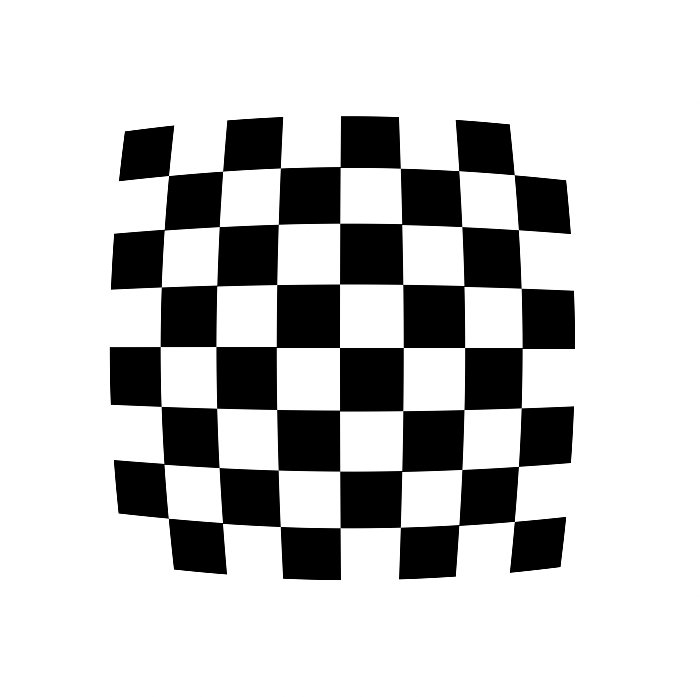
\includegraphics[trim = -10mm -10mm -10mm -10mm, width=0.35\textwidth]{figures/chess_input_3} }
  \subfloat[Output image]{ \label{fig:chess-3-o} 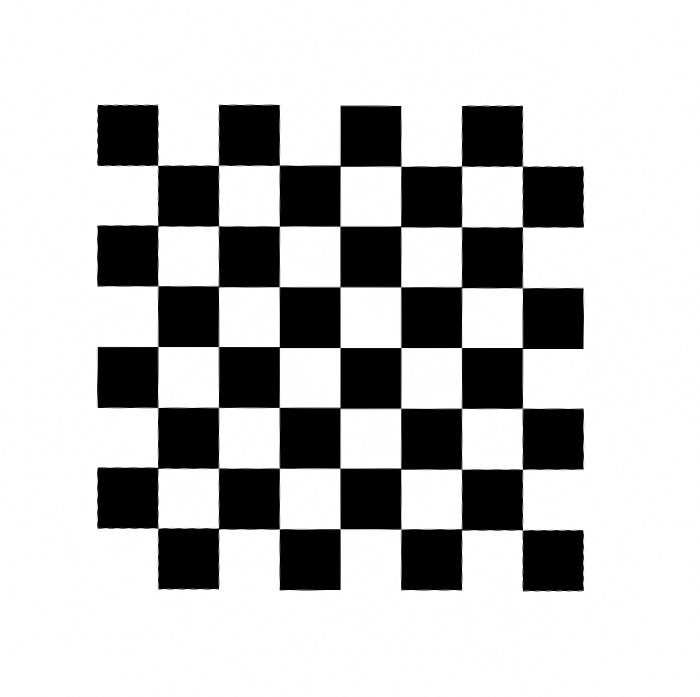
\includegraphics[trim = -10mm -10mm -10mm -10mm, width=0.35\textwidth]{figures/chess_output_3} }
  \caption{Artificial chessboard \#3: barrel distortion.}
  \label{fig:chess-3}
\end{figure}

\begin{figure}
  \centering
  \subfloat[Input image]{ \label{fig:chess-4-i} 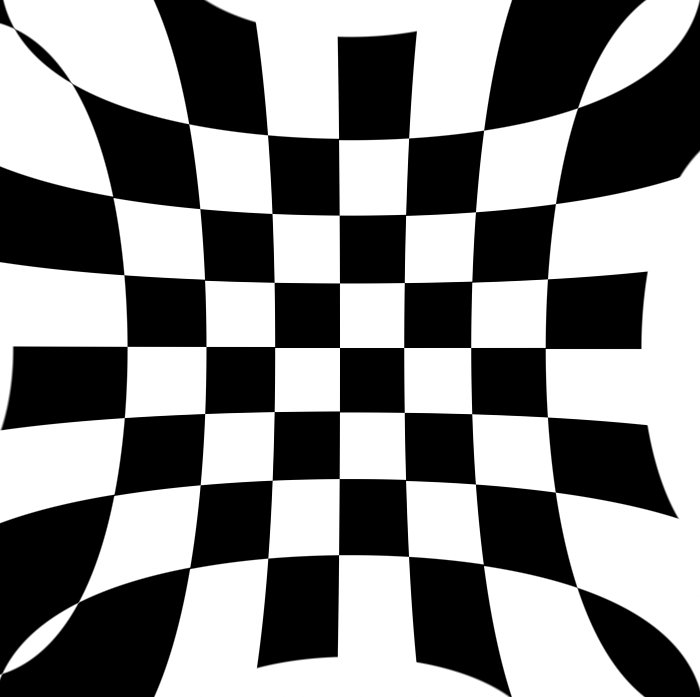
\includegraphics[trim = -10mm -10mm -10mm -10mm, width=0.35\textwidth]{figures/chess_input_4} }
  \subfloat[Output image]{ \label{fig:chess-4-o} 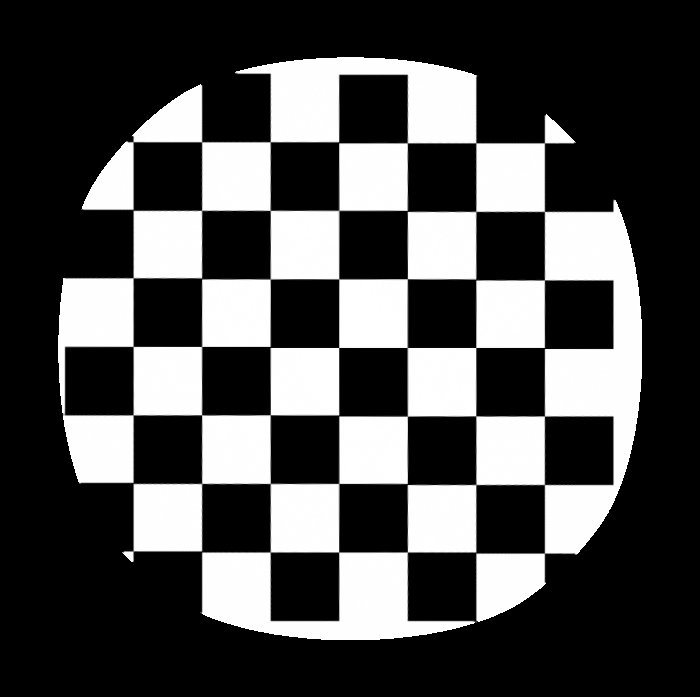
\includegraphics[trim = -10mm -10mm -10mm -10mm, width=0.35\textwidth]{figures/chess_output_4} }
  \caption{Artificial chessboard \#4: pincushion distortion.}
  \label{fig:chess-4}
\end{figure}

\begin{figure}
  \centering
  \subfloat[Input image]{ \label{fig:chess-8-i} 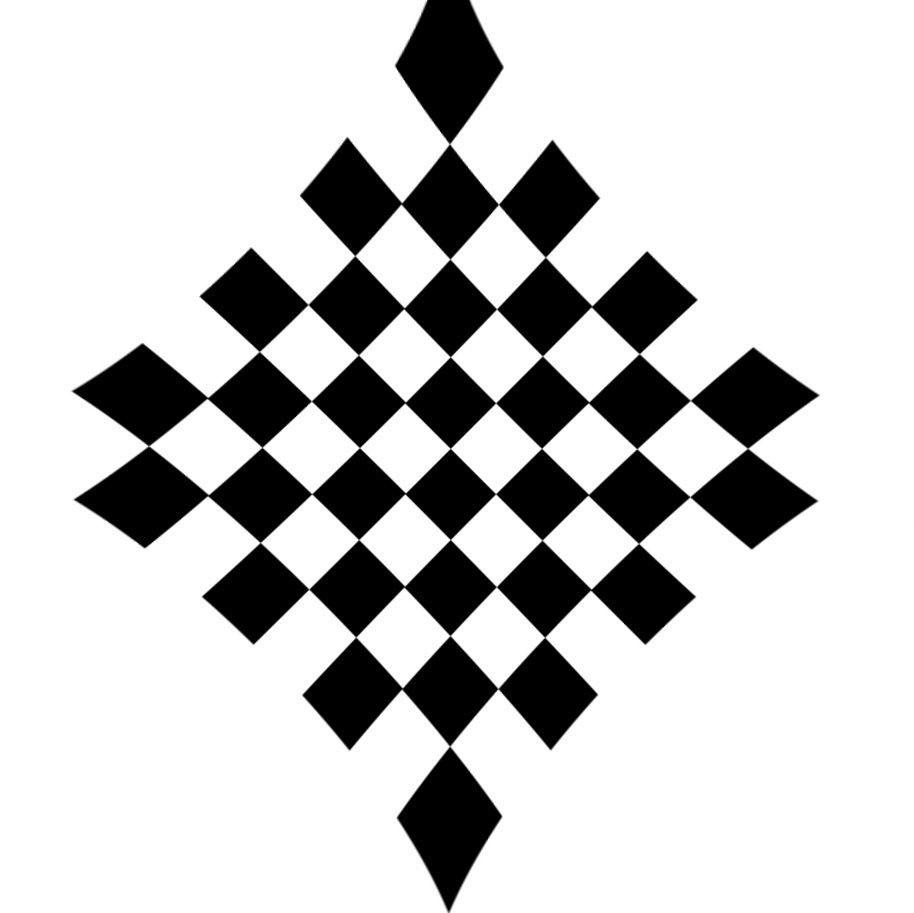
\includegraphics[trim = -10mm -10mm -10mm -10mm, width=0.35\textwidth]{figures/chess_input_8} }
  \subfloat[Output image]{ \label{fig:chess-8-o} 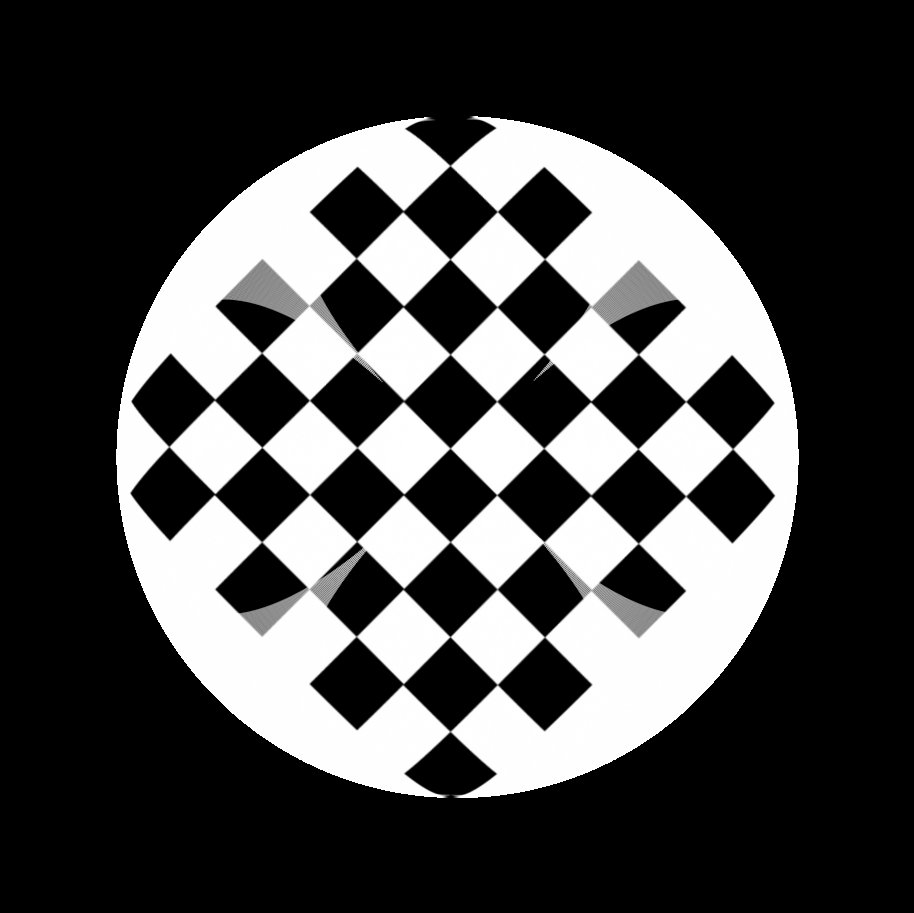
\includegraphics[trim = -10mm -10mm -10mm -10mm, width=0.35\textwidth]{figures/chess_output_8} }
  \caption{Artificial chessboard \#8: rotated pincushion distortion.}
  \label{fig:chess-8}
\end{figure}

\begin{figure}
  \centering
  \subfloat[Input image]{ \label{fig:chess-15-i} 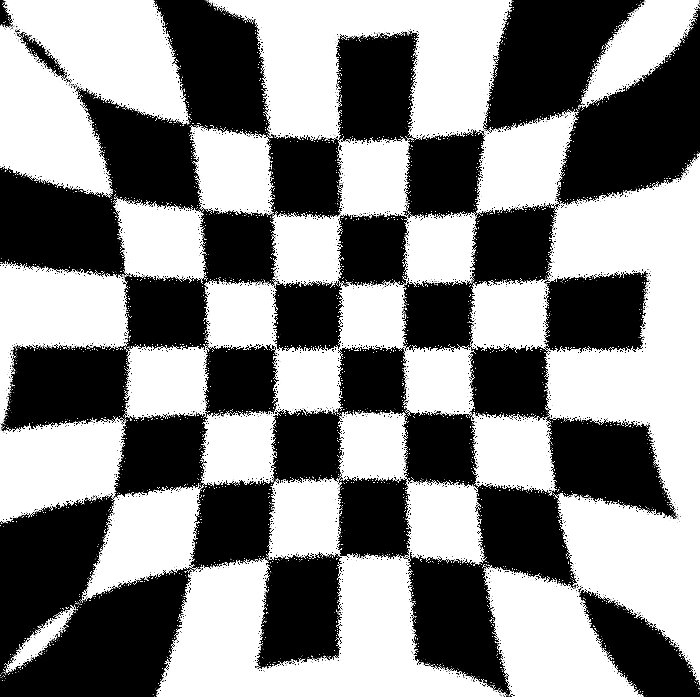
\includegraphics[trim = -5mm -5mm -5mm -5mm, width=0.3\textwidth]{figures/chess_input_15} }
  \subfloat[First output image]{ \label{fig:chess-15-o1} 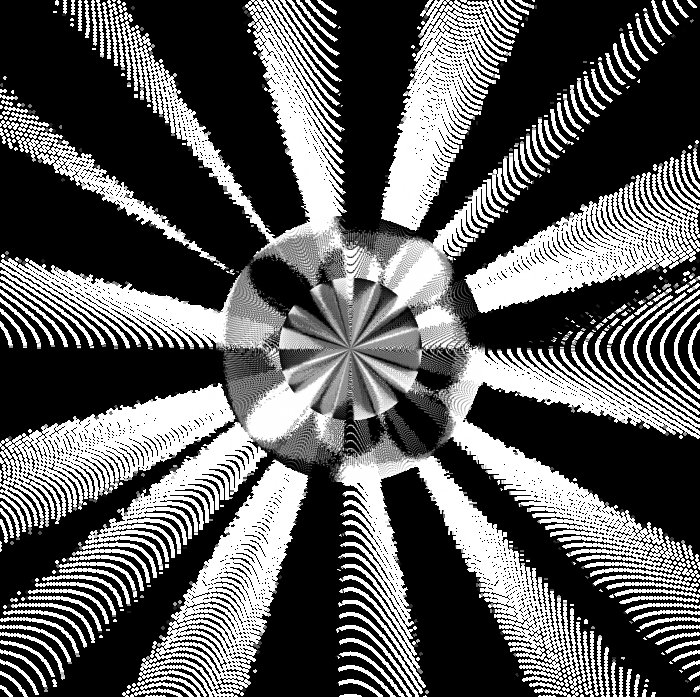
\includegraphics[trim = -5mm -5mm -5mm -5mm, width=0.3\textwidth]{figures/chess_output_15a} }
  \subfloat[Second output image]{ \label{fig:chess-15-o2} 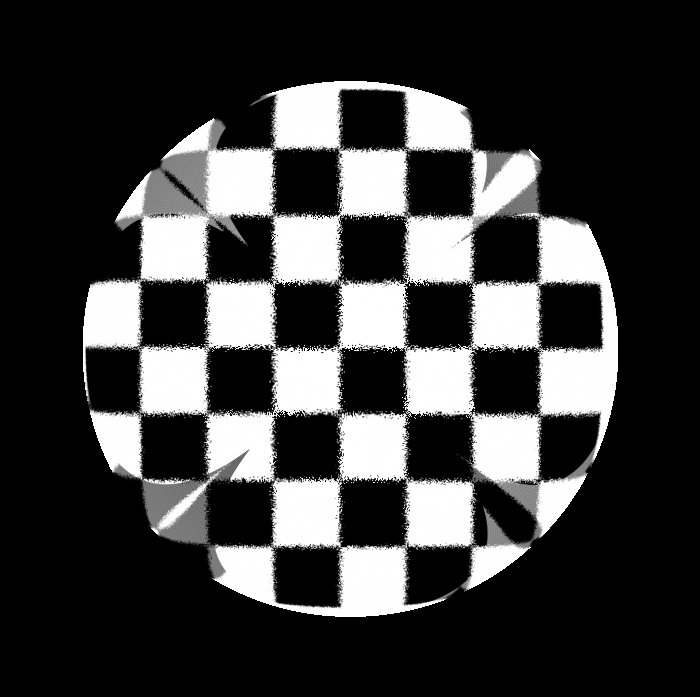
\includegraphics[trim = -5mm -5mm -5mm -5mm, width=0.3\textwidth]{figures/chess_output_15b} }
  \caption{Artificial chessboard \#15: pincushion distortion with $10\%$ spread noise.}
  \label{fig:chess-15}
\end{figure}

\begin{figure}
  \centering
  \subfloat[Input image]{ \label{fig:chess-19-i} 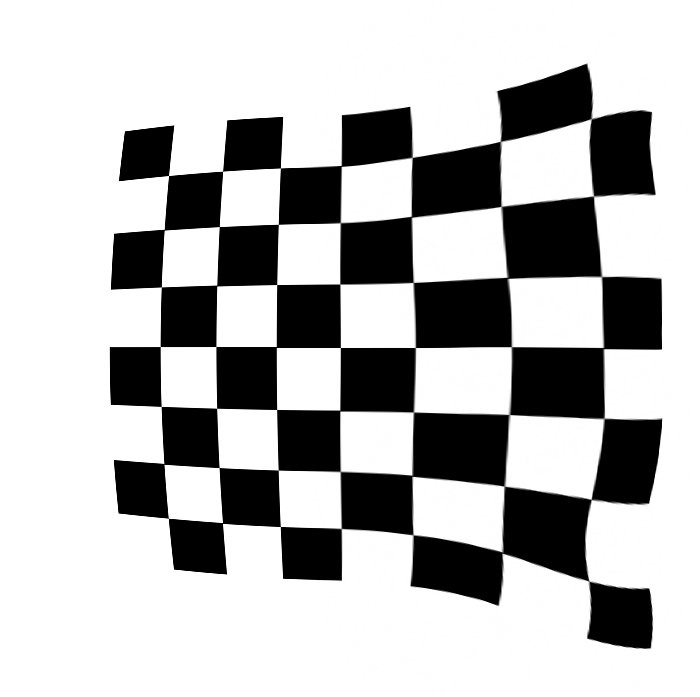
\includegraphics[trim = -10mm -10mm -10mm -10mm, width=0.35\textwidth]{figures/chess_input_19} }
  \subfloat[Output image]{ \label{fig:chess-19-o} 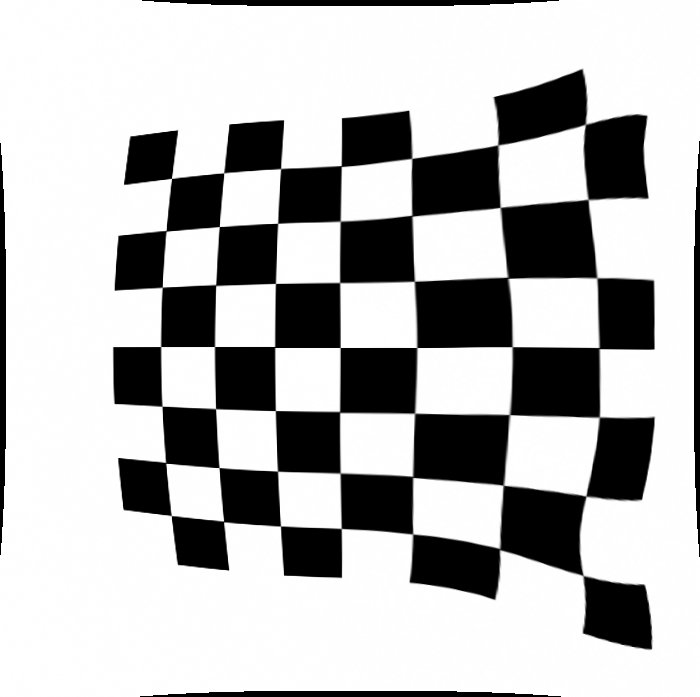
\includegraphics[trim = -10mm -10mm -10mm -10mm, width=0.35\textwidth]{figures/chess_output_19} }
  \caption{Artificial chessboard \#19: barrel distortion with stretched edge.}
  \label{fig:chess-19}
\end{figure}

\begin{figure}
  \centering
  \subfloat[Input image]{ \label{fig:chess-21-i} 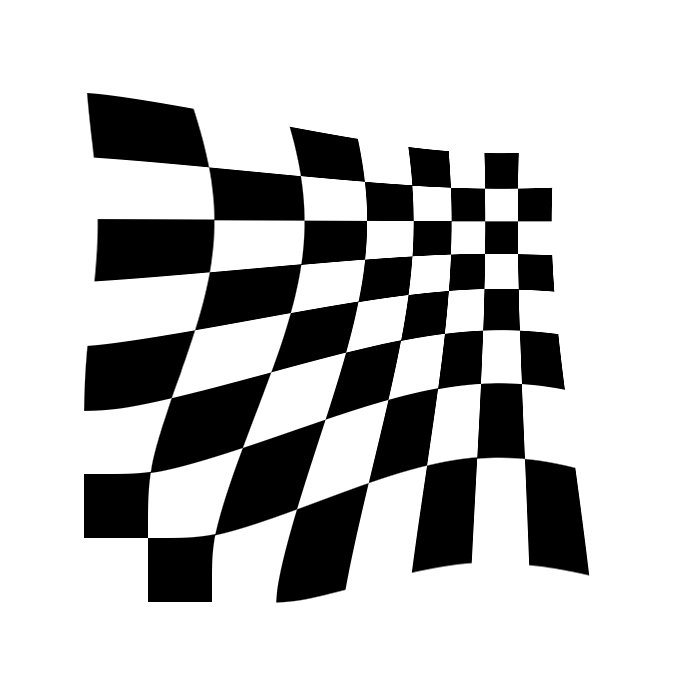
\includegraphics[trim = -10mm -10mm -10mm -10mm, width=0.35\textwidth]{figures/chess_input_21} }
  \subfloat[Output image]{ \label{fig:chess-21-o} 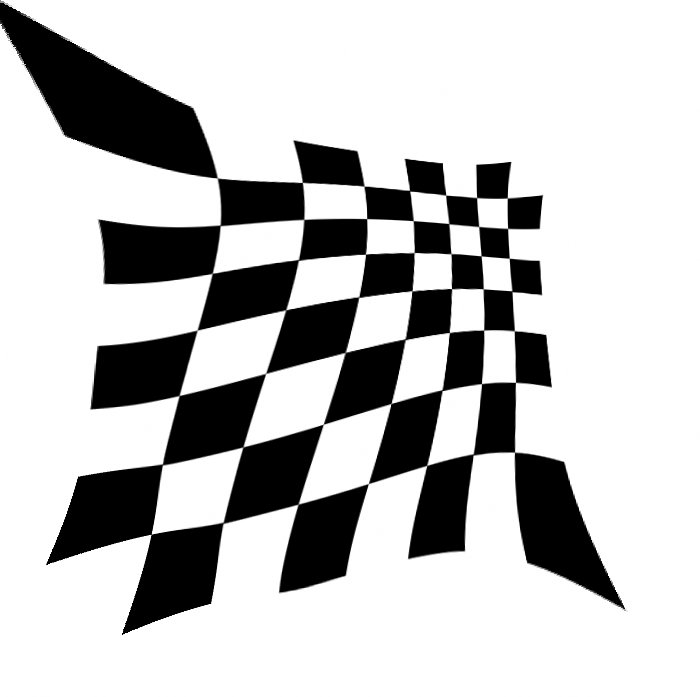
\includegraphics[trim = -10mm -10mm -10mm -10mm, width=0.35\textwidth]{figures/chess_output_21} }
  \caption{Artificial chessboard \#21: pseudo-pincushion distortion in one chessboard quadrant.}
  \label{fig:chess-21}
\end{figure}

\paragraph{Other tests.}
We also ran our program on a wide range of pseudo-chessboard images obtained in various ways: from internet searches, created by hand from distorted grids drawn by hand, or created by hand from distorted grids acquired from internet searches. These tests confirmed our results from running the program on our artificial chessboard suite. We confirmed that images of chessboards of strange dimensionalities (such as 4x10 or 14x16) can still be corrected, assuming the sizes of the chessboard squares are reasonable. We noted that the algorithm often cannot handle extreme camera angles or unusual types of noise (such as ``ink blotch" style noise, or significant noise at the corner-points of chessboard squares).

\subsubsection{Comparison with camera calibration results}

The process of camera calibration also involves determining the lens distortion parameters of the camera used to create an image. We now test our results with Tsai calibration from section~\ref{sec:calibration}. We took an image of the distortion object, and the images of its artificially barrel-distorted and pincushion-distorted variants, and generated lists of lines for each. These lines were created from the image calibration points, which ought to lie on straight lines on each face. For each of the three images, we used all horizontal lines on each face as well as the two outer vertical lines from each face, for a total of 18 lines per image. We ran the IPOLdistortion library directly on these, and compared the $\kappa_{0}$, $\kappa_{2}$, and $\kappa_{4}$ coefficients that were output to the $\kappa_{1}$ found by Tsai calibration.

\begin{table}[htb]
  \centering
  \begin{tabular}{| l | c c c | c |}
    \hline
    {\textbf{ }} &
    {\textbf{$\kappa_{0}$ (IPOL)}} &
    {\textbf{$\kappa_{2}$ (IPOL)}} &
    {\textbf{$\kappa_{4}$ (IPOL)}} &
    {\textbf{$\kappa_{1}$ (Tsai)}}\\
    \hline
    {\textbf{Normal}} & { } & { } & { } & { } \\
    {\textbf{calibration}} & {$1.0063$} & {$-2.746 \times 10^{-08}$} & {$1.926 \times 10^{-14}$} & {$-1.513 \times 10^{-08}$} \\
    {\textbf{image}} & { } & { } & { } & { } \\
    \hline
    {\textbf{Barrel}} & { } & { } & { } & { } \\
    {\textbf{-distorted}} & {$0.9659$} & {$9.536 \times 10^{-08}$} & {$3.814 \times 10^{-14}$} & {$1.194 \times 10^{-07}$} \\
    {\textbf{image}} & { } & { } & { } & { } \\
    \hline
    {\textbf{Pincushion}} & { } & { } & { } & { } \\
    {\textbf{-distorted}} & {$1.0583$} & {$-1.389 \times 10^{-07}$} & {$-6.806 \times 10^{-15}$} & {$-1.731 \times 10^{-06}$} \\
    {\textbf{image}} & { } & { } & { } & { } \\
    \hline
  \end{tabular}
  \caption[Comparison of Tsai calibration and IPOLdistortion lens distortion models]{Comparison of Tsai calibration and IPOLdistortion lens distortion models. The first three columns give the $\kappa_{0}$, $\kappa_{2}$, and $\kappa_{4}$ coefficients determined by the distortion removal code. The fourth column gives the $\kappa_{1}$ coefficient found by Tsai calibration.}
  \label{tbl:calib-distort-compare}
\end{table}

The results are presented in table~\ref{tbl:calib-distort-compare}. The distortion models are not immediately comparable, obviously, because the mathematical model developed by \cite{algebraic-distortion} ranges over even $\kappa$ values, whereas our implementation of Tsai calibration only calculates $\kappa_{1}$.

However, we can observe that both forms of distortion modelling have the lowest $\kappa$ coefficients for the normal image, with distortion increasing for the barrel-distorted image, and increasing significantly more (by as much as an order of magnitude) for the pincushion-distorted image. For all three image variations, the $\kappa_{1}$ calculated in Tsai calibration is closest to the $\kappa_{2}$ of IPOLdistortion - in magnitude and in sign. This is expected, given that both these $\kappa$ values are calculated by optimisation from the value $0$, whereas $\kappa_{0}$ (which might otherwise be considered equally close to $\kappa_{1}$) is calculated in the IPOLdistortion algorithm by optimisation from the value $1$.

We have seen that the results of the two algorithms are within the same "ballpark area". Although we lacked the testing apparatus to say so definitively, it is almost certain that the IPOLdistortion is the better distortion corrector, given our qualitative confirmation of the success of the IPOLdistortion algorithm on test images, and the simplistic (single $\kappa$) nature of the distortion model calculated as part of our Tsai calibration. However, one important caveat to remember, as \cite{straightlines} points out, is that images with too high distortion (e.g. actual ``fish-eye distortion") may not be suitably modelled at all using the polynomial $\kappa$-coefficients model.
